\documentclass[tikz,border=10pt]{standalone}
\usepackage{amsmath,amssymb}
\usetikzlibrary{calc,arrows.meta}

\begin{document}
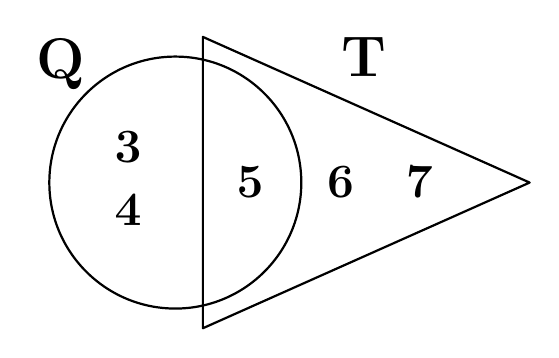
\begin{tikzpicture}[>=latex, line cap=round, line join=round]
  % Define Circle Q
  \def\r{1.6}
  \coordinate (O) at (0, 0);

  % Define Triangle T vertices
  \coordinate (Ttop) at (0.35, 1.85);
  \coordinate (Tbot) at (0.35, -1.85);
  \coordinate (Tapex) at (4.5, 0);

  % Draw Circle Q
  \draw[thick] (O) circle (\r);

  % Draw Triangle T
  \draw[thick] (Ttop) -- (Tapex) -- (Tbot) -- cycle;

  % Set labels with clean breathing margin
  \node at (-1.45, 1.5) {\huge $\mathbf{Q}$};
  \node at (2.4, 1.6) {\huge $\mathbf{T}$};

  % Elements inside Q only (stacked 3 and 4)
  \node at (-0.6, 0.45) {\LARGE $\mathbf{3}$};
  \node at (-0.6, -0.35) {\LARGE $\mathbf{4}$};

  % Element in intersection Q cap T
  \node at (0.95, 0.0) {\LARGE $\mathbf{5}$};

  % Elements inside T only (horizontal 6 and 7)
  \node at (2.1, 0.0) {\LARGE $\mathbf{6}$};
  \node at (3.1, 0.0) {\LARGE $\mathbf{7}$};

\end{tikzpicture}
\end{document}
